% Тут используется класс, установленный на сервере Papeeria. На случай, если
% текст понадобится редактировать где-то в другом месте, рядом лежит файл matmex-diploma-custom.cls
% который в момент своего создания был идентичен классу, установленному на сервере.
% Для того, чтобы им воспользоваться, замените matmex-diploma на matmex-diploma-custom
% Если вы работаете исключительно в Papeeria то мы настоятельно рекомендуем пользоваться
% классом matmex-diploma, поскольку он будет автоматически обновляться по мере внесения корректив
%

% По умолчанию используется шрифт 14 размера. Если нужен 12-й шрифт, уберите опцию [14pt]
\documentclass[14pt]{matmex-diploma}
%\documentclass[14pt]{matmex-diploma-custom}

\usepackage{listings}
\usepackage{minted}
\usepackage{verbments}
\usepackage{algpseudocode}
\usepackage{algorithm}
\usepackage{caption}
\usepackage{algorithmicx}
\usepackage{amssymb}


\begin{document}

\renewcommand{\lstlistingname}{Листинг}
\renewcommand\listingscaption{Листинг}


% Год, город, название университета и факультета предопределены,
% но можно и поменять.
% Если англоязычная титульная страница не нужна, то ее можно просто удалить.
\filltitle{ru}{
    chair              = {Фундаментальная информатика и информационные технологии \\ Профиль Математическое и программное обеспечение вычислительных машин, комплексов и компьютерных сетей},
    title              = {Ослабленный синтаксический анализ динамически формируемых выражений на основе алгоритма GLL},
    % Здесь указывается тип работы. Возможные значения:
    %   coursework - Курсовая работа
    %   diploma - Диплом специалиста
    %   master - Диплом магистра
    %   bachelor - Диплом бакалавра
    type               = {master},
    position           = {студента},
    group              = 661,
    author             = {Рагозина Анастасия Константиновна},
    supervisorPosition = {к.\,ф.-м.\,н., доц.},
    supervisor         = {Булычев Д.\,Ю.},
    reviewerPosition   = {ООО "ИнтеллиДжей Лабс" \\ инженер-программист},
    reviewer           = {Шкредов С.\,Д.},
    chairHeadPosition  = {д.\,ф.-м.\,н., профессор},
    chairHead          = {Новиков Б.\,А.},
%   university         = {Санкт-Петербургский Государственный Университет},
%   faculty            = {Математико-механический факультет},
%   city               = {Санкт-Петербург},
%   year               = {2013}
}
\filltitle{en}{
    chair              = {Fundamental Computer Science and Information Technologies \\ Software of Computers, Complexes and Networks},
    title              = {GLL-based relaxed parsing of dynamically generated code},
    author             = {Ragozina Anastasiya},
    supervisorPosition = {assistant professor},
    supervisor         = {Dmitri Boulytchev},
    reviewerPosition   = {IntelliJ Labs Co. Ltd \\ Software Developer},
    reviewer           = {Sergey Shkredov},
    chairHeadPosition  = {professor},
    chairHead          = {Novikov B.},
    type               = {master} 
}
\maketitle
\tableofcontents
% У введения нет номера главы
\section*{Введение}
При работе с формальными языками и грамматиками выводимость цепочки в грамматике можно рассматривать как следующее свойство: цепочка $\omega$ обладает свойством $S$ , если $\omega$ выводима из $S$: ($S \Rightarrow^* \omega $). При решении практических задач, как правило, выполняют проверку свойства выводимости в грамматике для отдельно взятых цепочек, либо же для конечного множества цепочек, представленных в явном виде (например, в виде множества файлов с исходным текстом программ). На практике такие множества могут оказаться бесконечными, что делает такую проверку невозможной. Подобная ситуация может возникнуть, если цепочки генерируются автоматически. Множество порождаемых генератором цепочек в этом случае будет регулярным. Для описания регулярных множеств часто используются конечные автоматы. Таким образом возникает задача проверки свойства выводимости в КС-грамматике для всех элементов множества, заданного конечным автоматом. Такую задачу будем называть синтаксическим анализом регулярных множеств. 
	
Описанная задача имеет практическое применение и возникает в ряде областей. Например, широкое распространение при разработке информационных систем получил подход, использующий динамически формируемые программы. Код таких программ формируется в процессе выполнения внешней программы из строковых литералов и в дальнейшем выполняется соответствующим окружением. Такой подход может использоваться для генерации SQL-запросов, Web-страниц, запросов к XML-подобным структурам данных. Однако, проблема заключается в том, что динамически формируемый код не подвергается статической проверке стандартными инструментами, так как компилятором он воспринимается как обычные строки. Статический анализ встроенного кода позволил бы выявлять ошибки до того, как программа будет запущена. Кроме того, общепринятой практикой при разработке информационных систем является использование интегрированных сред разработки, которые упрощают процесс разработки путём подсветки синтаксиса, автодополнения и других функций. Для встроенных языков подобные возможности также были бы полезны. Для решения таких задач необходимо иметь структурное представление кода (дерево разбора), которое строится в процессе синтаксического анализа. При этом задача анализа динамически формируемого кода осложняется тем, что все возможные значения программы нельзя задать простым перечислением. Это происходит из-за того, что для формирования кода могут использоваться циклы, потенциально бесконечные. Для представления такого кода можно построить регулярную аппроксимацию сверху, представленную в виде конечного автомата над алфавитом встроенного языка. Таким образом мы приходим к задаче синтаксического анализа регулярных множеств при обработке динамически формируемого кода. Важной особенностью задач в данной области является необходимость построения дерева разбора, что выдвигает дополнительные требования к алгоритму анализа.

Другим примером использования синтаксического анализа регулярных множеств является поиск подпоследовательностей генома (таких как РНК, например) в задачах биоинформатики. Для того, чтобы классифицировать образцы, взятые из окружающей среды, для них строится метагеномная сборка, являющаяся комбинацией генов всех организмов, находящихся в образце. Сборка представляется в виде графа с последовательностями символов на рёбрах. В таком графе необходимо найти подстроки, позволяющие провести классификацию. Искомые подстроки могут быть описаны КС-грамматикой~\cite{Anderson}, то есть необходимо искать подстроки, обладающие свойством выводимости. В данном случае не обязательно строить дерево разбора, необходимо лишь ответить на вопрос: порождается ли цепочка данным автоматом. Данная задача может быть решена с помощью синтаксического анализа регулярных множеств.

Анализу динамически формируемых программ посвящён ряд работ~\cite{LrAbstract1, LrAbstract2, LRAbstractParsingSema}.  Изучению данной проблемы посвящена также работа~\cite{RelaxedARNGLR}, в которой описан алгоритм анализа встроенных языков с использованием алгоритма RNGLR, строящий структурное представление динамически формируемого кода. Однако в этой работе указано, что у предложенного решения существуют проблемы с производительностью. Синтаксический анализа также применяется в задачах биоинформатики, однако только для линейных входных данных. При этом отдельное внимание необходимо уделять производительности решения. Это обуславливается тем, что входные данные при анализе метагеномной сборки, как правило, имеют очень большой размер: порядка $10^5$ рёбер, $10^5$ вершин, $10^8$ --- суммарная длина символов в метках рёбер. 
		
\section{Постановка задачи}
Целью данной работы является создание решения для синтаксического анализа регулярных множеств, применимого для работы со входными данными большого размера. Для достижения поставленной цели были поставлены следующие задачи.

\begin{itemize}  
\item Разработать алгоритм синтаксического анализа динамически  формируемого кода на основе алгоритма GLL. 
\item Доказать корректность предложенного алгоритма.
\item Применить к задаче поиска на входных данных большого размера.
\item Реализовать предложенный алгоритм в рамках проекта \\ YaccConstructor.
\item Произвести эксперименты и сравнение.
\end{itemize}

\section{Обзор}
%\subsection{Основные определения из области формальных языков}
\subsection{Обобщённый синтаксический анализ}
Большинство языков программирования могут быть описаны однозначной КС-грамматикой, но создание такой грамматики является трудоёмким и долгим процессом. На практике, как правило, спецификацию необходимо получить быстро, по этой причине доступная для разработчиков спецификация языка часто содержит неоднозначности. Приведение грамматики к детерминированной форме --- процесс сложный, часто приводящий к появлению ошибок. Для работы с неоднозначными грамматиками используются алгоритмы обобщённого синтаксического анализа. Такие алгоритмы рассматривают все возможные пути разбора входной цепочки и строят все деревья вывода для неё.

Впервые такой подход был предложен в работе~\cite{Tomita}: на основе алгоритма восходящего синтаксического анализа LR был разработан алгоритм GLR. Такой алгоритм позволил обрабатывать конфликты типа shift/reduce и reduce/reduce, которые не могут быть корректно обработаны обычными LR-анализаторами. Принцип работы GLR-алгоритма остался таким же, как и у LR-алгоритма, но для заданной грамматики GLR-парсер строит все возможные выводы входной последовательности, используя поиск в ширину. В ячейках LR-таблиц хранится не более одного правила свёртки для текущего символа во входном потоке. В ячейках таблицы GLR-парсера может храниться несколько правил свёртки. Эта ситуация соответствует конфликту типа reduce/reduce. Когда возникает конфликт, т.е. символ на входе может быть разобран несколькими разными способами, стек парсера разветвляется на два или больше параллельных стека. Верхние состояния этих стеков соответствуют возможным переходам. Если для какого-либо верхнего состояния и входного символа в таблице не существует ни одного перехода, то эта ветка разбора считается ошибочной и отбрасывается. 

Позже было предложено множество модификаций GLR-алгоритма: RIGLR~\cite{RIGLR}, RNGLR, BRNGLR~\cite{BRNGLR}. Восходящие анализаторы в отличие от нисходящих, как правило, имеют сложную структуру и трудны для разработки. В 2010 году был предложен алгоритм обобщённого анализа Generalised LL (GLL)~\cite{GLL} на основе алгоритма нисходящего синтаксического анализа. Основная идея осталась прежней --- просмотр всех возможных путей разбора и ветвление стека в случае возникновения неоднозначностей. В силу особенностей работы LL-алгоритма соответствующие анализаторы более просты для разработки, и, кроме того, они имеют более высокую скорость работы.

Прежде чем переходить к описанию процесса работы алгоритма, рассмотрим принцип работы синтаксических анализаторов, созданных с помощью метода рекурсивного спуска (Recursive Descent, RD). RD-анализаторы являются процедурной интерпретацией грамматики. Их непосредственная связь с грамматикой упрощает их разработку, отладку и внесение изменений при необходимости. Рассмотрим простую грамматику $G_0$ (листинг~\ref{grmG0}) и соответствующий анализатор, написанный методом рекурсивного спуска.

\begin{listing}
\caption{Грамматика $G_0$}
\label{grmG0}
\centering
$\begin{array}{rl}
s & \rightarrow a \ b \ | \ b \ C \\
b & \rightarrow A \ | \ C \\
a & \rightarrow A 
\end{array}$
\end{listing}

Анализатор, созданный с помощью метода рекурсивного спуска, для данной грамматики будет состоять из функций для разбора нетерминалов --- $parseS()$, $parseB()$, $parseA()$, и управляющей процессом разбора функции main(). Но поскольку данная грамматика не является однозначной, разбор даже корректного входа, например, цепочки {\it ``ac''}, будет заканчиваться ошибкой. Кроме того, в худшем случае время работы таких парсеров может экспоненциально зависеть от размера входа для сильнонеоднозначных грамматик. 

Алгоритм Generalised LL является обобщением алгоритмов LL и рекурсивного спуска и способен обрабатывать все контекстно свободные грамматики, в том числе содержащие левую рекурсию. Как и в классическом рекурсивном спуске, в GLL-анализаторах сохраняется тесная связь с грамматикой, что упрощает  реализацию и отладку. Вместе с этим, расход памяти и время работы в худшем случае является кубическим относительно размера входа и линейным для LL-грамматик. Это обеспечивается за счёт использования специализированных структур данных хранения стека и леса разбора.

\subsection{Структурированный в виде графа стек}
Стек в алгоритмах синтаксического анализа используется для того, чтобы запоминать ранее разобранные символы. Поскольку алгоритмы обобщённого синтаксического анализа строят все возможные выводы входной строки, необходимо для каждого варианта разбора хранить свой стек. Как только в процессе разбора происходит конфликт, создаётся несколько новых процессов анализа и каждый из них будет иметь свой собственный стек. Каждый такой стек будет иметь общую часть и разным у них будет только верхнее состояние. Проблема данного подхода заключается в том, что хранение отдельных стеков в явном виде требует слишком больших накладных расходов. Для того, чтобы бороться с этим, стеки комбинируются с помощью структуры данных GSS (Graph Structured Stack). В результате всё множество стеков представляется в виде графа, а в качестве вершины конкретного стека можно хранить только указатель на соответствующую вершину графа. На рис.~\ref{GSS} показан пример объединения нескольких стеков: для стеков S1, S2 и S3 в результате будет получен S1.

\begin{figure}
 \centering
 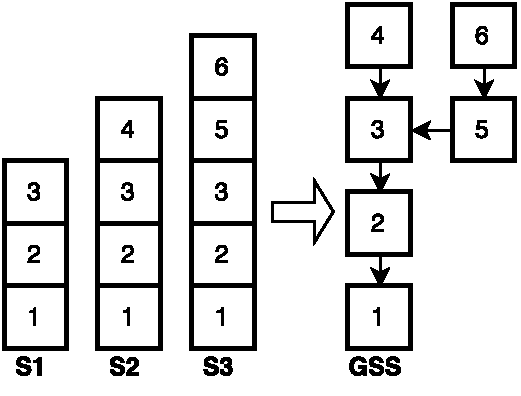
\includegraphics[width=8cm]{pics/GSS.pdf}
 \caption{Стек, структурированный в виде графа  }
 \label{GSS}
\end{figure}

В вершине GSS хранится правило грамматики с указанием позиции в правой части (обозначается $X \rightarrow \alpha x \cdot \beta$, дальше просто \textit{слот}) и позиция во входном потоке. Позиция во входном потоке используется для того, чтобы различать вершины стека. На ребре GSS хранится часть леса разбора, построенное на соответствующем шаге работы анализатора. Описанное представление GSS обладает существенным недостатком: многие вершины и рёбра дублируются. Для примера рассмотрим грамматику $G_1$ (листинг~\ref{grmG1}).

\begin{listing}
\caption{Грамматика $G_1$}
\label{grmG1}
\centering
$\begin{array}{rl}
a \rightarrow A \ a \ B \ | \ A \ a \ C \ | \ A
\end{array}$

\end{listing}
Для такой грамматики в процессе разбора будет построен GSS (в дальнейшем просто стек), показанный на рис. 2({\it а}). На рисунке видно, что рёбра дублируются. Этот же стек может быть представлен как показано на рис. 2({\it б}). Таким образом можно значительно уменьшить размер графа без потери информации. 

\begin{figure}
 \centering
 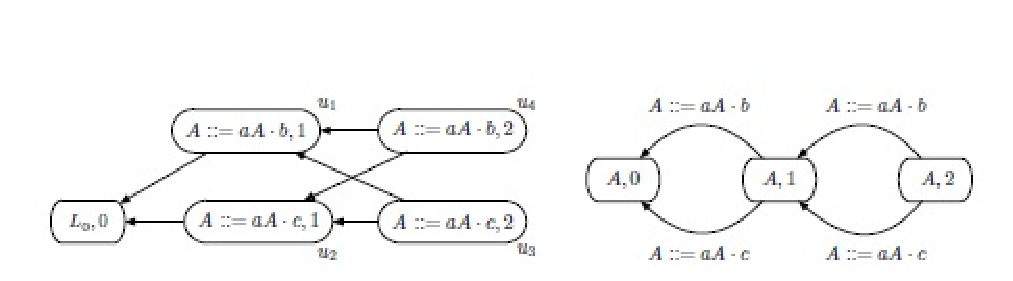
\includegraphics[width=15cm]{pics/GSSNew.pdf}
 \caption{{\it а} --- старая версия GSS;  {\it б} --- модифицированный GSS }
 \label{GSS2}
\end{figure}

Данная модификация стека предложена в работе~\cite{Afroozeh2015}, посвященной улучшению производительности работы алгоритма GLL. Уменьшение количества рёбер в стеке достигается за счёт хранения в вершинах не слота целиком, а только имени нетерминала и позиции во входном потоке. Соответствующий слот в описанном варианте хранится на ребре стека. В конечном итоге уменьшение количества вершин и рёбер позволяет значительно ускорить время работы алгоритма и уменьшить объём потребляемой памяти~\cite{Afroozeh2015}. В данной работе были использованы эти результаты.

\subsection{Сжатое представление леса разбора}
Результатом работы синтаксического анализатора является дерево разбора. Для неоднозначных грамматик для одной и той же входной цепочки может быть построено несколько различных деревьев, для некоторых грамматик количество деревьев может экспоненциально зависеть от размера входа. Для того, чтобы уменьшить количество требуемой для хранения деревьев памяти, используется структура данных Shared Packed Parse Forests (SPPF)~\cite{SPPF}, которая позволяет хранить лес разбора более компактно. Это достигается за счёт того, что в SPPF узлы с одинаковыми деревьями под ними переиспользуются, а узлы, которые соответствуют разным выводам одной и той же цепочки из одного и того же нетерминала, комбинируются. Например, для сильно неоднозначной грамматики $G_2$ (листинг~\ref{grmG2}) и входной цепочки  {\it ``bbb''} может быть построено два дерева, показанных на рис.~\ref{SPPF1}{\it (a)} и рис. ~\ref{SPPF1}{\it (б)}, которые могут быть сжаты в SPPF так, как показано на рис.~\ref{SPPF1}{\it (в)}.

\begin{listing}
\caption{Грамматика $G_2$}
\label{grmG2}
\centering
$\begin{array}{rl}
s \rightarrow s \ s \ | \ B
\end{array}$
\end{listing}

\begin{figure}
 \centering
 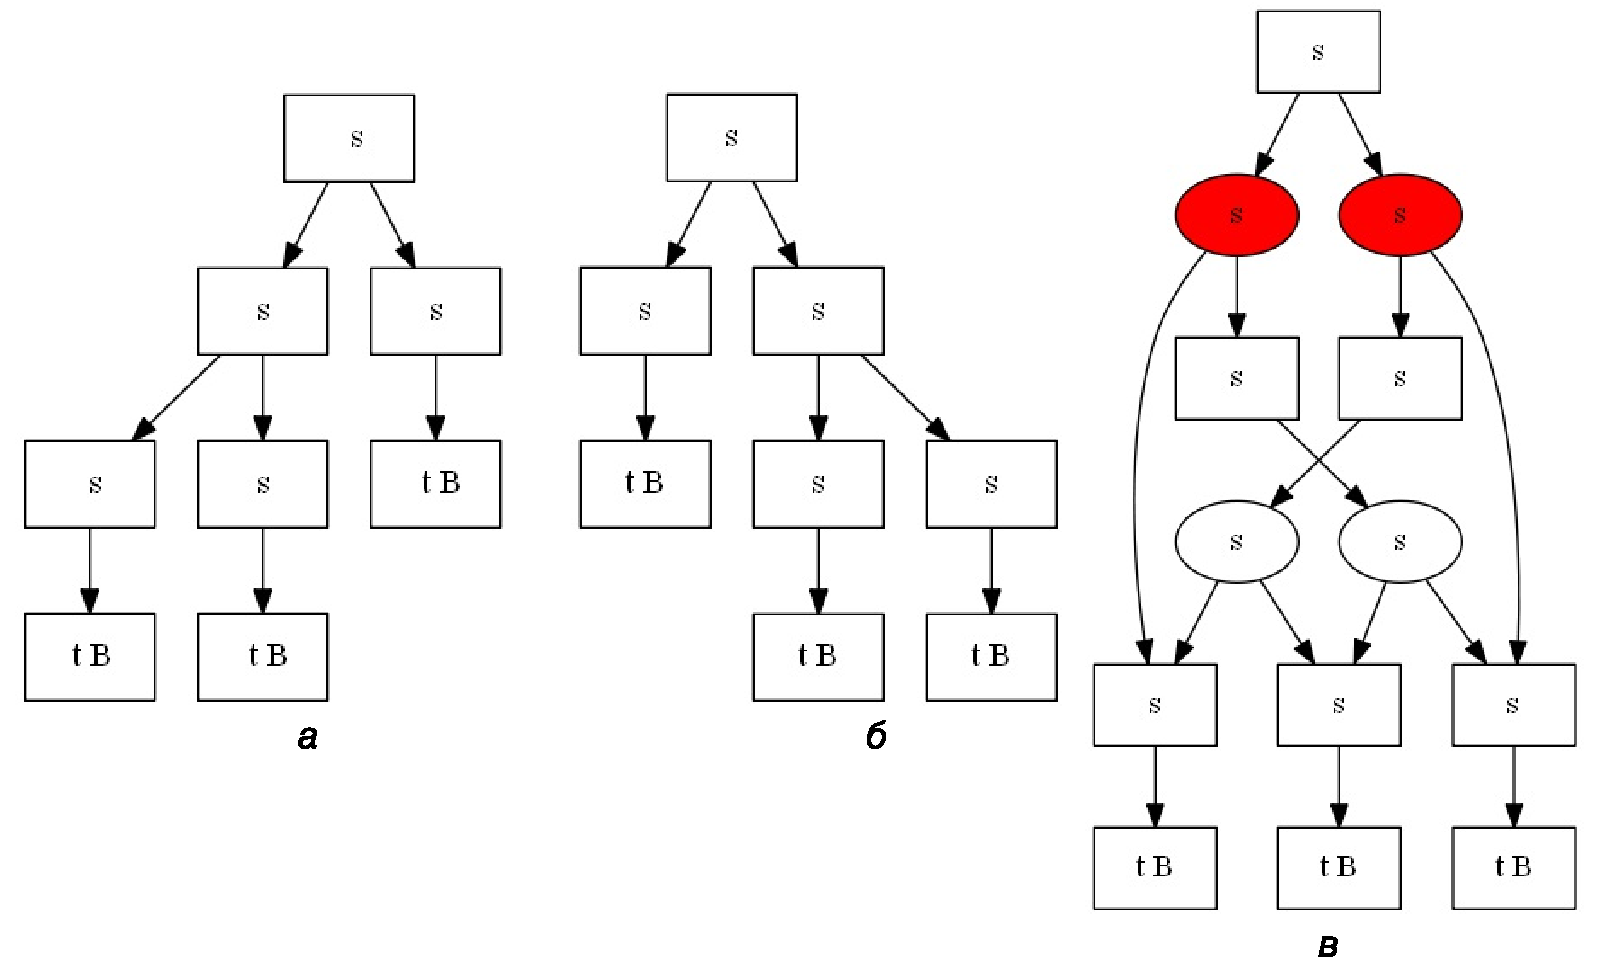
\includegraphics[width=15cm]{pics/SPPF1.pdf}
 \caption{{\it а} --- левый вывод; {\it б} --- правый вывод; {\it в} --- сжатое представление леса разбора }
 \label{SPPF1}
\end{figure}

В алгоритме GLL строится бинаризированная версия SPPF, в которой используется три типа узлов --- символьные, упакованные и промежуточные узлы. Символьные узлы представляют собой тройку $(x, i , j)$, где $х$ имя нетерминала или терминала (различают, соответственно, терминальные и нетерминальные узлы), а $i$ и $j$ --- позиции во входном потоке, которым соответствует рассматриваемая часть дерева (для корня --- узла, помеченного стартовым нетерминалом, --- начальной позицией будет 0, а конечной длина строки). Позиции во входном потоке дальше будем называть правой и левой координатами узла. Промежуточные узлы хранят слот и позиции во входном потоке. Упакованные узлы имеют вид ($ a \rightarrow \gamma \cdot, k$), где $k$ --- правая позиция для левого сына, которая используется для того, чтобы различать узлы. Терминальные узлы не имеют потомков и являются листьями в SPPF. Нетерминальные и промежуточные узлы могут иметь несколько потомков, упакованные узлы имеют только оного или двух, где правым потомком является символьный узел вида $(x, k, i)$, а левым, если существует, --- символьный или промежуточный узел вида $(s, j, k)$. Упакованные узлы используются для описания фактов неоднозначности в выводе, т.е. если у нетерминала более одного упакованного узла в потомках, то для этого нетерминала было построено несколько выводов одной и той же цепочки. На рис.~\ref{SPPF2} изображен SPPF для грамматики $G_2$.

\begin{figure}
 \centering
 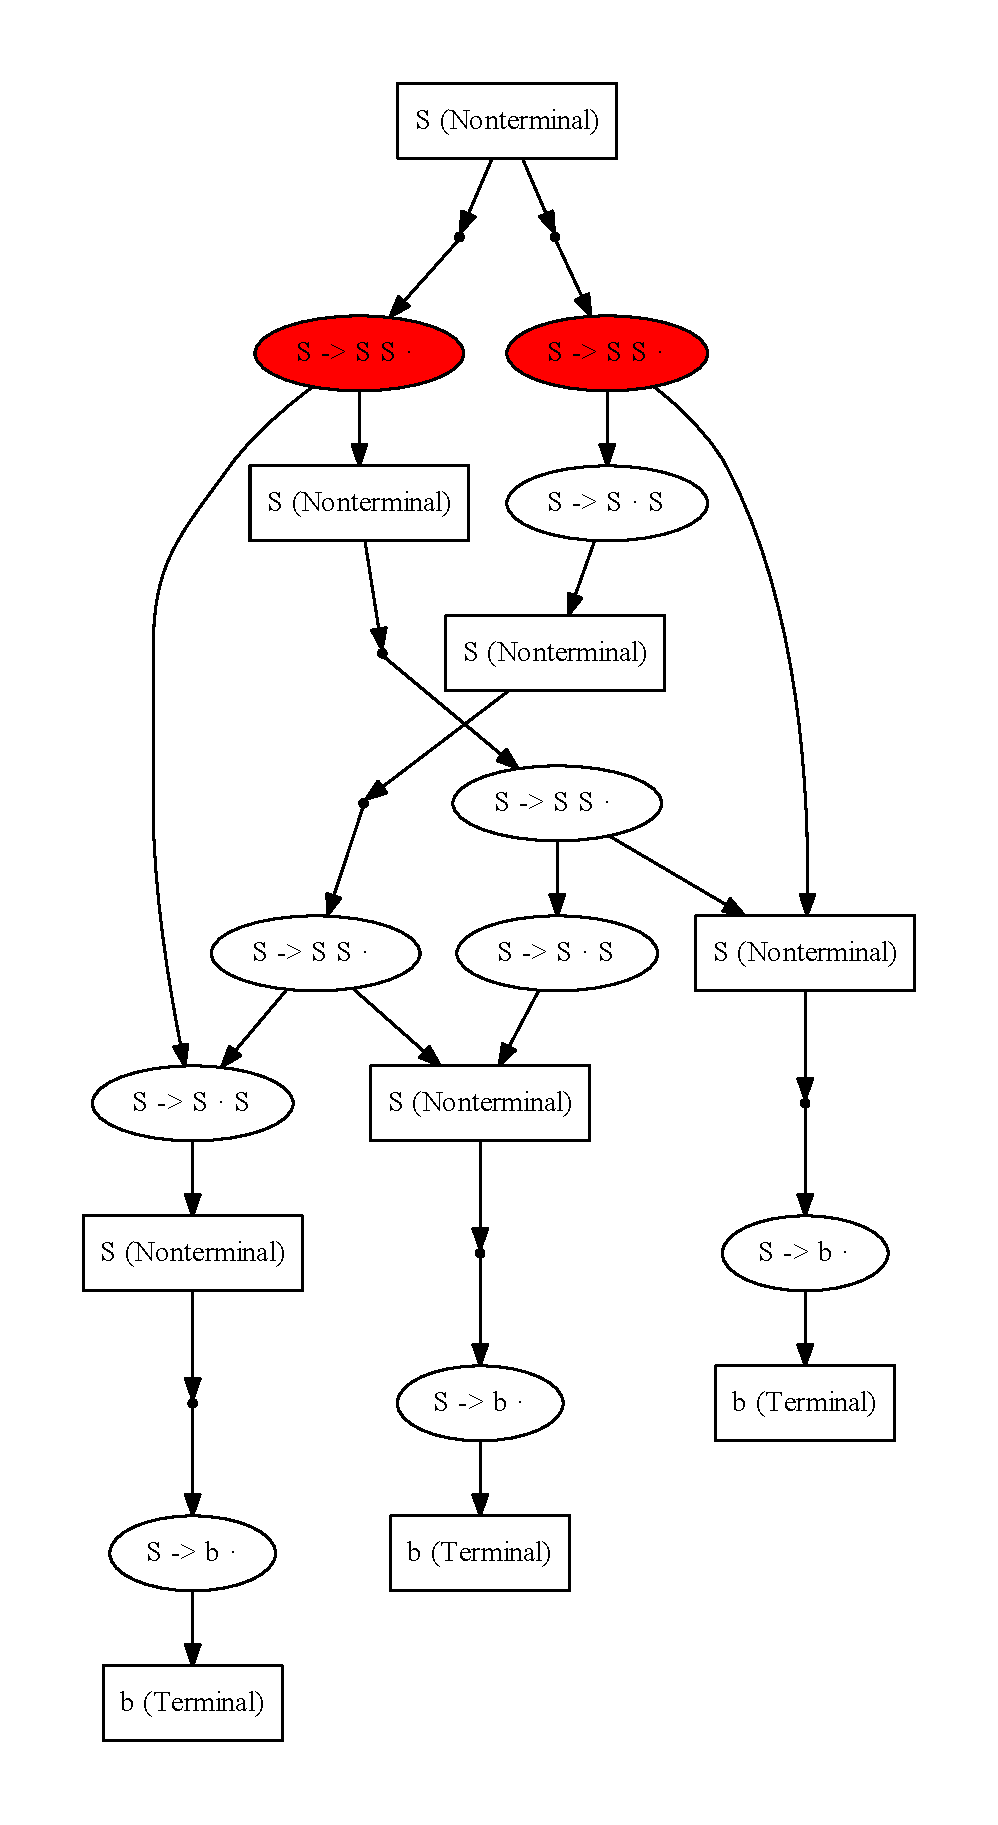
\includegraphics[width=10cm]{pics/GLLSppf.pdf}
 \caption{Бинаризированное представление сжатого леса разбора для грамматики $G_2$ и входной строки {\it ``bbb''} }
 \label{SPPF2}
\end{figure}

На рис.~\ref{SPPF2} точками обозначены упакованные узлы. Узлы, помеченные слотами, являются промежуточными, а терминальные и нетерминальные узлы подписаны. У стартового нетерминала имеется два потомка, что свидетельствует о существовании двух выводов для данной входной цепочки.

\subsection{Алгоритм GLL}
Процесс работы GLL-анализатора можно рассматривать как обход грамматики в соответствии со входным потоком. На каждом шаге выполнения GLL анализатор находится в некоторой позиции в грамматике вида $x \rightarrow \alpha X \cdot \beta$, которая обозначается $L$, и поддерживает три переменные: текущая позиция во входном потоке (cI), текущая вершина стека (cU) и текущий узел в дереве (cN). Эта четвёрка называется дескриптором и позволяет полностью описать текущий шаг разбора. Дескрипторы извлекаются из очереди и разбор каждый раз начинается заново с точки, описанной в дескрипторе. Если какой-то путь не может быть продолжен, то процесс анализа не заканчивается ошибкой: вместо этого из очереди извлекается следующий дескриптор и процесс возобновляется с точки, описанной в нём. Алгоритм останавливается, как только очередь дескрипторов становится пустой.

Синтаксический анализатор состоит из набора функций с уникальными метками, управление между которыми передаётся с помощью оператора \texttt{goto()}. В отличии от парсеров, созданных с помощью метода рекурсивного спуска, в GLL-анализаторах функции генерируется для каждой альтернативы и у \texttt{goto()} может быть несколько целевых меток. Функции бывают двух видов: для каждой альтернативы нетерминала, соответствующие слотам в грамматике вида $a \rightarrow \cdot\gamma$, и функциями для слотов вида $ y \rightarrow \delta x \cdot \mu$. При создании дескриптора в качестве текущей позиции в грамматике запоминается имя целевой функции. Кроме того, имеется управляющая функция, которая извлекает очередной дескриптор из очереди и вызывает соответствующую функцию с помощью операции \texttt{goto()}. Также есть функция для построения стека \texttt{create()} и для построения дерева \texttt{getNodeP()} и \texttt{getNodeT()}. Функция \texttt{getNodeT()} используется для создания терминального узла, а \texttt{getNodeP()} для создания всех остальных видов узлов.

Стек частично заменяет вызов функции в парсерах, написанных методом рекурсивного спуска. Вершины стека создаются, как только в процессе обхода грамматики встречается нетерминал (например, $x \rightarrow \alpha \cdot a \beta$). Как упоминалось ранее, на вершинах стека находятся пары $(N, i)$, где $N$ --- имя нетерминала, который необходимо разобрать, $i$ --- позиция во входном потоке на момент создания вершины. На ребре хранится слот и часть леса разбора. Слот позволяет сохранить информацию о том, в какую позицию в грамматике необходимо вернуться после того, как нетерминал будет разобран (в случае слота $x \rightarrow \alpha a \cdot \beta$ разбирается нетерминал a). Второй элемент пары --- часть леса разбора, которая была построена на момент создания вершины стека (для рассматриваемого слота $x \rightarrow \alpha a \cdot \beta$ это часть SPPF для цепочки $\alpha$). После того, как нетерминал будет разобран, вершина извлекается из стека и для всех исходящих рёбер создаются новые дескрипторы $(l, i, u, t)$, где $l$ --- слот с ребра, $i$ --- текущая позиция во входном потоке, $u$ --- целевая вершина ребра и $t$ --- часть леса разбора, полученная объединением части леса с ребра и построенной для нетерминала (для рассматриваемого слота $x \rightarrow \alpha a \cdot \beta$ объединяется часть леса для цепочки $\alpha$ и нетерминала $A$).

\begin{listing}
\caption{Грамматика $G_3$}
\label{grmG3}
\centering
$\begin{array}{rl}
s \rightarrow A \ s \ B \ | \ D \ | \ A \ D \ B 
\end{array}$
\end{listing}

Кроме того, для корректной работы алгоритма используются дополнительные множества. Все дескрипторы добавляются в очередь $R$ и последовательно извлекаются из неё в процессе работы анализатора. Процесс работы синтаксического анализатора недетерминирован и может возникнуть ситуация, когда один и тот же дескриптор будет создаваться снова и снова. Повторное создание дескриптора приводит к тому, что процесс зациклится и никогда не завершится. Для того, чтобы избежать дублирования дескрипторов, отдельно хранится множество $U$ ранее созданных дескрипторов. В очередь добавляются только дескрипторы, не содержащиеся во множестве $U$. Для того, чтобы хранить и переиспользовать уже разобранные нетерминалы используется множество $P$. В нём хранятся пары вида $(u; z)$, где $z$ --- узел SPPF, а $u$ --- вершина GSS. Ниже приведён пример GLL-анализатора для грамматики $G_3$. В приведённом примере функция $L_0$ содержит основной цикл, который извлекает дескрипторы из очереди и присваивает переменным cU, cI  и cN значения из извлечённого дескриптора. 

\begin{figure}
 \centering
 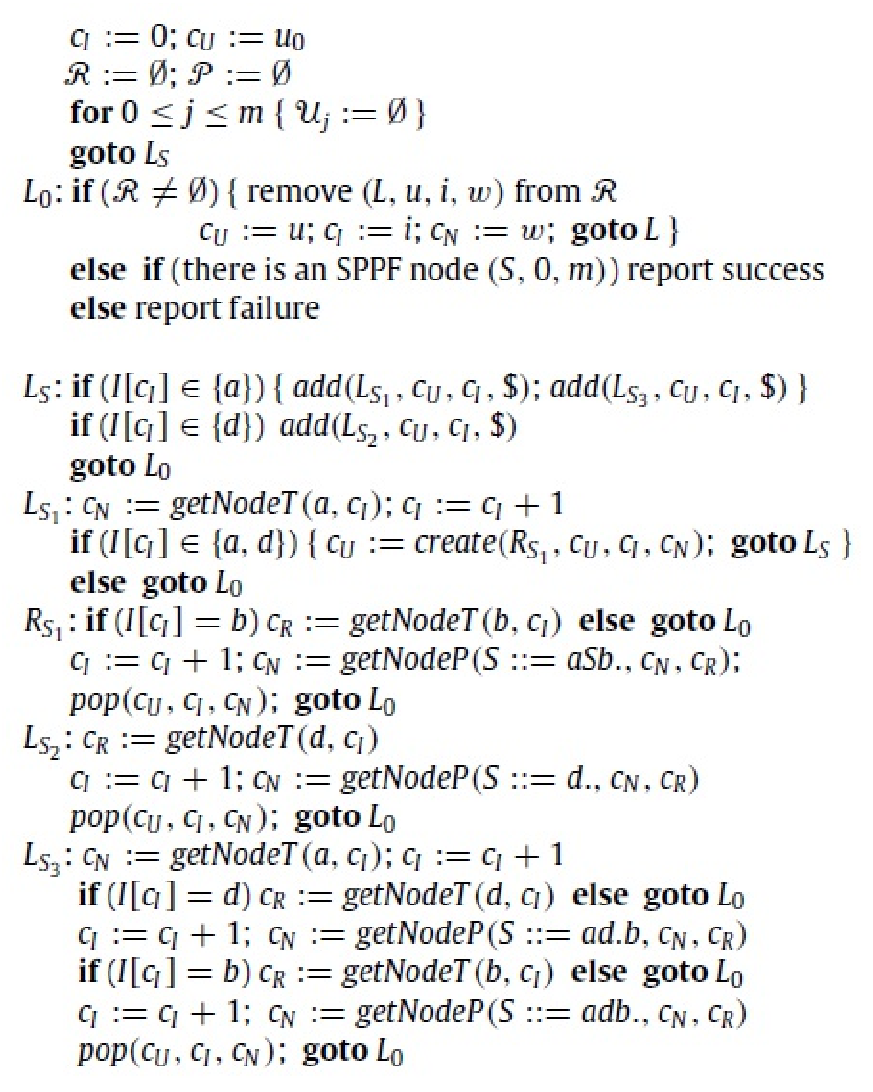
\includegraphics[width=10cm]{pics/Listing1.pdf}
 \label{ListingGLL1}
 \caption{GLL-анализатор для грамматики $G_3$ }
\end{figure}

\subsection{Подходы к анализу встроенных языков}
В области анализа встроенных языков ведутся исследования и разрабатываются инструменты, реализующие различные подходы. 
\begin{itemize}
\item Java String Analyzer (JSA)~\cite{JSA,JSAUrl} --- инструмент для анализа строк и строковых операций в программах на Java. Основан на проверке включения регулярной аппроксимации встроенного языка в контекстно-свободное описание эталонного языка.
\item PHP String Analyzer (PHPSA)~\cite{PHPSA,PHPSAUrl} --- инструмент для статического анализа строк в программах на PHP. Расширяет подход инструмента JSA. В инструменте уточнена проводимая аппроксимация и это повышает точность проводимого анализа. 
\item Alvor~\cite{AlvorUrl, Alvor2, Alvor1} --- плагин к среде разработки Eclipse, предназначенный для статической проверки корректности SQL-выражений, встроенных в Java. Для компактного представления множества динамически формируемого строкового выражения используется понятие абстрактной строки, которая, фактически, является регулярным выражением над используемыми в строке символами. В инструменте Alvor отдельным этапом выделен лексический анализ. Поскольку абстрактную строку можно преобразовать в конечный автомат, то лексический анализ заключается в преобразовании этого конечного автомата в конечный автомат над терминалами при использовании конечного преобразователя, полученного генератором лексических анализаторов JFlex. Несмотря на то, что абстрактная строка позволяет описывать строковые выражения при конструировании которых использовались циклы, плагин в процессе работы выводит сообщение о том, что данная языковая конструкция не поддерживается. Также инструмент Alvor не поддерживает обработку строковых операций, за исключением конкатенации, о чём также выводится сообщение во время работы.
\item IntelliLang~\cite{IntelliLang} --- плагин к средам разработки IntelliJ IDEA и PHPStorm, предоставляющий поддержку встроенных строковых языков, таких как HTML, SQL, XML, JavaScript в указанных средах разработки. Данное расширение обеспечивает подсветку синтаксиса, автодополнение, статический поиск ошибок. Для среды разработки IntelliJ IDEA расширение IntelliLang также предоставляет отдельный текстовый редактор для работы со встроенным языком. Для использования данного плагина требуется ручная разметка переменных, содержащих выражения на том или ином встроенном языке.
\item Varis~\cite{Varis} --- плагин для Eclipse, представленный в 2015 году и предоставляющий поддержку кода на HTML, CSS и JavaScript, встроенного в PHP. В плагине реализованы функции подсветки встроенного кода, автодополнения, перехода к объявлению (jump to declaration), построения графа вызовов (call graph) для встроенного JavaScript. 
\end{itemize}

Все эти инструменты предназначены для решения достаточно узких задач и часто не предусматривают проведения сложного анализа динамически формируемого кода. Более сложные виды анализа могут быть произведены с применением абстрактного синтаксического анализа, который предложен в работе~\cite{LrAbstract2}. Алгоритм абстрактного синтаксического анализа комбинирует анализ потока данных и синтаксический LR-анализа. Входными данными для него является набор data-flow уравнений, описывающих множество значений динамически формируемого кода. Данные уравнения решаются в домене LR-стеков при помощи абстрактной интерпретации~\cite{AbstractInterpretation}, обеспечивающей свойство завершаемости алгоритма. Результатом работы является набор абстрактных синтаксических деревьев, которые в дальнейшем могут использоваться для решения различных задач статического анализа. К сожалению, в работах отсутствует рассмотрение эффективного представление результатов анализа. Кроме того, инструментов, реализующих предложенный подход, в открытом доступе нет.

Также существует подход к обработке динамически формируемого кода,  основанный на алгоритме обобщённого восходящего анализа RNGLR~\cite{RelaxedARNGLR}. Подход основан на проверке включения регулярного языка в некоторые подклассы КС-языков. В качестве входных данных в работе используется регулярное приближение множества всех значений динамически формируемого кода в некоторой точке программы-генератора. Данное приближение описывается регулярным языком $L$ и является приближением сверху (over-approximation) для множества возможных значений: регулярный язык содержит все предложения, генерируемые программой и, возможно, ещё какие-то. Благодаря этому можно говорить о достоверности многих видов статического анализа. Таким образом, регулярная аппроксимация для множества значений динамически формируемых выражений позволяет решать многие важные задачи, например, поиск ошибок во встроенном коде. Для представления регулярной аппроксимации используются конечные автоматы, так как для любого регулярного языка $L$ можно построить конечный автомат, такой что он принимает те и только те цепочки, которые принадлежат языку $L$. Далее построенный конечный автомат подаётся на вход лексическому анализу (преобразуется из автомата над символами в автомат над токенами), а затем синтаксическому анализу, алгоритм которого основан на алгоритме RNGLR. Достоинствами предложенного решения являются модульность, позволяющая рассматривать различные этапы анализа отдельно, и возможность построения конечного леса вывода для всех корректных цепочек из $L$, что позволяет реализовывать различные виды анализа динамически формируемого кода, требующие его структурного представления.

\subsection{YaccConstructor}
YaccConstructor~\cite{YCUrl} --- исследовательский проект лаборатории языковых инструментов JetBrains, направленный на изучение алгоритмов лексического и синтаксического анализа. Проект включает в себя одноимённый модульный инструмент с открытым исходным кодом, предоставляющий платформу для разработки лексических и синтаксических анализаторов, содержащую большое количество готовых компонент, таких как различные преобразования грамматик, язык описания атрибутных грамматик YARD и др. Большинство компонент реализованы на платформе .NET, основным языком разработки является F\# ~\cite{FSharp}. Предоставляемый язык спецификации грамматик YARD, поддерживает атрибутные грамматики, грамматики в расширенной форме Бэкуса-Наура и многое другое.

В рамках проекта была создана платформа для статического анализа динамически формируемого кода, основанная на модульной архитектуре, предложенной в~\cite{GrigorievPhd}. В рамках соответствующих модулей реализованы механизмы лексического анализа, описанный в~\cite{polubelova}, и алгоритм синтаксического анализа, описанный в~\cite{RelaxedARNGLR}. Благодаря модульной архитектуре, данные компоненты могут использоваться независимо. 

\subsection{Анализ метагеномной сборки}
В биологических исследованиях часто необходимо ответить на вопрос, к какому виду относится тот или иной организм. Образцы часто берутся из окружающей среды и могут быть не идентифицированы. По таким образцам строится метагеномная сборка, являющаяся множеством участков ДНК различных организмов. Такое множество может быть представлено в виде конечного автомата, порождающего геномы всех организмов, содержащихся в образце. Саму последовательность ДНК можно рассматривать, как строку в алфавите $\{A, C, G, T\}$, однозначно определяющую организм (или штамм), к которому она относится. 

Наиболее часто используемый подход для идентификации образцов, взятых из окружающей среды, --- проведение сравнительного анализа последовательности рРНК. Поскольку большая часть информации об организме хранится именно в рРНК. При этом для поиска и идентификации подцепочек используется несколько основных механизмов: скрытые цепи Маркова, используемые в таких инструментах, как HMMER~\cite{hmmer}, REAGO~\cite{reago}, ковариационые модели (covariation model, CM)~\cite{durbin}, основанные на вероятностных грамматиках и применении синтаксического анализа для задачи поиска. Однако проблема заключается в том, что восстановление небольших участков рРНК по объёмной метагеномной сборке оказывается трудоёмким и не всегда её может быть решена эффективно. 

Существующие подходы для решения такой задачи можно разделить на два класса. Первый класс сначала использует инструменты для анализа сборок de novo (полные геномные последовательности организмов, находящихся в метагеномной сборке, ещё не известны), которые восстанавливают геномные последовательности в линейном виде. Затем результат их работы передаётся инструментам геномного поиска рРНК. Проблема данных инструментов заключается в том, что восстановление генов в метагеномной сборке задача очень трудоёмкая. Кроме того, большая часть генов de novo состоит из участков, не носящих информации о рРНК. Таким образом, подход построения метагеномой сборки и поиска рРНК по ней с использованием сторонних инструментов не оптимален. 

Другой класс инструментов реализует поиск непосредственно в метагеномной сборке. Часть из них используют предварительную фильтрацию отдельных линейных участков (предполагается, что сборка ещё не представлена в виде конечного автомата), что позволяет избавиться от анализа последовательностей, не несущих необходимой информации. Затем из оставшихся частей производится сборка pРНК. Такой подход используется в EMIRGE~\cite{Emirge}. Недостатком подхода является необходимость наличия большого числа известных рРНК и высокая вероятность не найти далеко стоящие друг от друга рРНК. Инструмент REAGO лишён этих проблем, однако он не работает с метагеномной сборкой, представленной в виде графа, а хранение сборки в виде набора прочитанных участков требует большого объёма памяти.

Обработка сборки, представленной в виде графа реализована в инструменте Xander~\cite{Wang2015}, который использует для решения задачи композицию скрытых моделей Маркова (HMM) и входного графа. Недостатком такого подхода является то, что использование HMM даёт существенно более низкую точность результата по сравнению с использованием CM~\cite{EddyComputationalRNA}. Наиболее известным инструментом, использующим CM для поиска рРНК является Infernal~\cite{Infernal}. Однако он не применим к метагеномным сборкам, представленным в виде графа.

\subsection{Выводы}
В результате выполненного обзора были сделаны следующие выводы.
\begin{enumerate}
\item Алгоритм синтаксического анализа, предложенный в работе~\cite{RelaxedARNGLR} позволяет решать задачу построения леса вывода для динамически формируемого кода. Поэтому идеи, предложенные в этих работах взяты за основу данной диссертации.
\item Алгоритм синтаксического анализа GLL имеет более очевидную связь с грамматикой, чем восходящие алгоритмы анализа, поддерживает произвольные КС-грамматики и обладает высокой производительностью, что позволяет использовать его для задач синтаксического анализа регулярных множеств.
\item YaccConstructor содержит готовое решение для синтаксического анализа динамически формируемого кода, основанное на RNGL-алгоритме. При этом архитектура этого решения позволяет легко заменять алгоритмы синтаксического анализа, оставляя без изменений другие компоненты, такие как лексический анализ, построение аппроксимации~\cite{SELforIDE}. Таким образом YaccConstructor является подходящей платформой для практической реализации.
\item Применение механизмов синтаксического анализа к конечным автоматам является важной задачей в биоинформатике.
\end{enumerate}

\section{Алгоритм анализа регулярных множеств}
Целью данной работы является создание алгоритма синтаксического анализа регулярных множеств, который может быть применим для анализа встроенных языков. Как упоминалось ранее, встроенный код порождается в момент выполнения основной программы. Для генерации могут использоваться строковые операторы, условные операторы и циклы из-за чего такой код не может быть представлен линейно. Результатом работы лексического анализатора на таком коде является не линейный поток токенов, а конечный автомат над алфавитом токенов. В рамках данной работы на такие автоматы накладывается следующее ограничение: они должны быть детерминированными. Если это условие не будет выполняться, то нельзя будет однозначно выбрать, по какому пути производить разбор. Например, для встроенного кода на листинге~\ref{lst:brExpr} будет построен конечный автомат на рис.~\ref{input}.

%\fvset{frame=lines,framesep=5pt}
\begin{listing}
\begin{pyglist}[language=csharp,numbers=left,numbersep=5pt]
 string expr = "" ;
 for(int i = 0; i < len; i++) 
 {
     expr = "()" + expr;
 }
\end{pyglist}
\caption{Код на C\#, динамически формирующий скобочную последовательность}
\label{lst:brExpr}
\end{listing}

\begin{figure}[h]
 \centering
 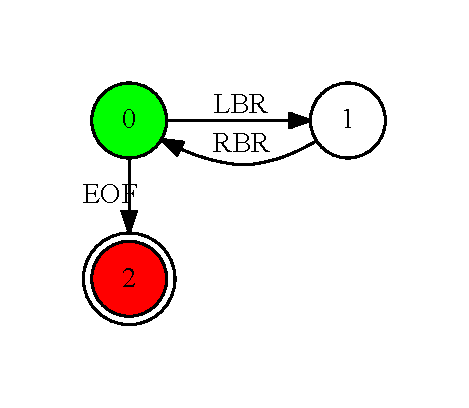
\includegraphics[width=5cm]{pics/input.pdf}
 \caption{Конечный автомат, представляющий аппроксимацию встроенного кода для листинга~\ref{lst:brExpr} }
 \label{input}
\end{figure}

В алгоритме вместо хранения позиции во входном потоке теперь хранится номер вершины во входном графе. Поскольку вход является нелинейным, то вместо того, чтобы просматривать один текущий входной символ на каждом шаге, рассматриваются все исходящие рёбра для текущей вершины и выбирается одно (как упоминалось ранее, автомат детерминирован, поэтому это возможно), соответствующее текущему терминальному символу в грамматике. Если такого ребра нет, то алгоритм просто продолжает свою работу --- из очереди достаётся новый дескриптор и процесс возобновляется. 

Для автоматического создания синтаксических анализаторов существует несколько подходов. В рамках первого подхода весь код парсера генерируется по грамматике. Чаще всего такой подход используется при генерации анализаторов, построенных методом рекурсивного спуска. При генерации нисходящих анализаторов для каждого нетерминала генерируются функции, которые последовательно вызываются в процессе разбора. Несмотря на то, что нисходящие анализаторы просты для разработки, и поэтому чаще всего создаются вручную, существуют инструменты для автоматической генерации таких анализаторов. Например, инструмент ANTLR~\cite{antlr} --- генератор парсеров, позволяющий автоматически создавать анализаторы на одном из целевых языков программирования по описанию LL(*)-грамматики на языке, близком к EBNF. Структура генераторов такого типа изображена на рис.~\ref{genTypes}{\it (а)}.

\begin{figure}
 \centering
 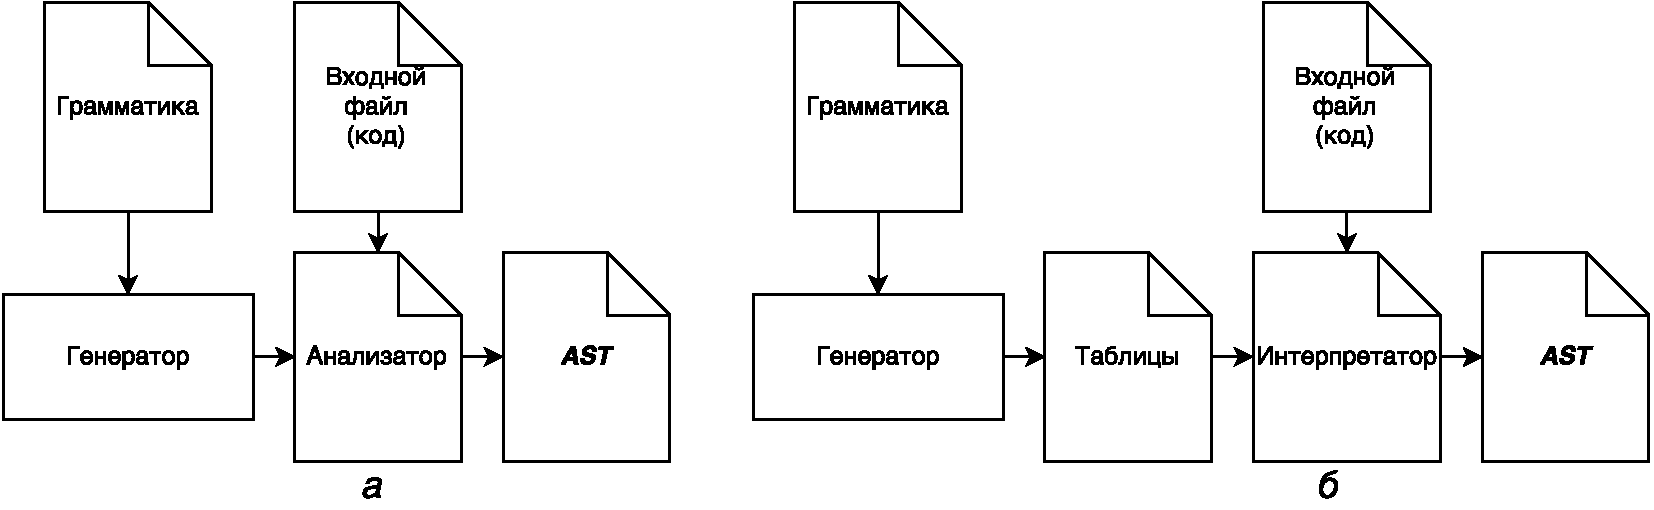
\includegraphics[width=15cm]{pics/GeneratorTypes.pdf}
 \caption{Подходы к генерации синтаксических анализаторов}
 \label{genTypes}
\end{figure}

Существует ещё один подход для генерации синтаксических анализаторов, который используется для получения табличных анализаторов. Отдельно создаётся интерпретатор, который содержит в себе основную логику алгоритма. Интерпретатор пишется вручную и переиспользуется. По грамматике каждый раз генерируется дополнительная информация, которая необходима интерпретатору в процессе работы. Структура такого генератора представлена на рис.~\ref{genTypes}{\it (б)}. Чаще всего в качестве дополнительной информации генерируются таблицы синтаксического анализа, управляющие процессом разбора.

В оригинальных работах, описывающих GLL-алгоритм, используется первый подход. В рамках данной работы был выбран второй подход из-за его гибкости и универсальности. Вместо генерации функций по слотам грамматики и их последовательного вызова, в главном цикле алгоритма просто рассматриваются все возможные состояния, в которых может находиться парсер. В зависимости от того, какой символ во входном потоке и какая позиция в грамматике, в процессе разбора рассматриваются следующие ситуации.

\begin{itemize}
\item Если текущий символ в грамматике является терминалом $x$ и существует исходящее из текущей вершины ребро, помеченное этим нетерминалом, то указатель в грамматике нужно сдвинуть на одну позицию вправо, $x \rightarrow \alpha X \cdot \beta$, и текущей вершиной назначить конечную вершину ребра. Никаких дополнительных действий со стеком при этом не производится. Иначе, если нет ребра, помеченного терминалом $х$, то текущая ветка разбора считается ошибочной, отбрасывается и  разбор продолжается с использованием следующего дескриптора.
\item Если текущий символ в грамматике является нетерминалом $a$, то необходимо в стек записать слот, по которому продолжить разбор после того, как правило для $a$ будет разобрано. Указатель в грамматике перемещается на $a \rightarrow \cdot \gamma $, а номер вершины во входном потоке остаётся без изменений.
\item Если указатель в грамматике имеет следующий вид $x \rightarrow \alpha\cdot$ и стек не пуст, то слот вида $y \rightarrow \delta x \cdot \mu$, который хранится в этот момент в текущей вершине стека, извлекается и становится текущим.
\item Если текущий слот имеет вид $s \rightarrow \tau\cdot$, и весь входной поток рассмотрен, то разбор завершается успешно, иначе разбор заканчивается ошибкой. В случае успешного завершения разбора возвращается дерево, иначе сообщение об ошибке.
\end{itemize}

Наличие циклов во входном графе никак не влияет на процесс разбора. Дескрипторы позволяют без каких-либо изменений процесса разбора обработать их. Это делает результирующий алгоритм более простым в отличие от алгоритма, основанного на RNGLR , в который потребовалось внести существенные изменения для поддержки циклов~\cite{RelaxedARNGLR}. За счёт того, что каждый раз при добавлении дескриптора выполняется проверка всей четвёрки целиком (позиция во входе, слот, вершина стека и часть леса разбора), то лишние дескрипторы с одинаковыми деревьями не создаются. Переиспользование уже созданных узлов также позволяет избежать создания лишних деревьев: если дерево с определёнными координатами и соответствующим правилом вывода уже было создано, то повторно такое дерево создаваться не будет.

В алгоритме так же поддерживается четвёрка: слот (вместо имени функции), номер вершины в графе, вершина стека и узел дерева. Поскольку вызов функций заменён на обработку ситуаций, возникающих в процессе анализа, в теле основной функции, то появилась необходимость определять, какое правило вывода использовать для разбора. Для определения правила используются LL-таблицы, где в каждой ячейке может быть несколько правил для разбора, что соответствует ситуации наличия в грамматике неоднозначностей. Анализатор состоит из функции, содержащей основной цикл алгоритма, функции управляющей процессом разбора и функций для построения дерева и стека.

\begin{listing}[H]
\hrule
\begin{algorithmic}
\caption{Функция, содержащая в себе основную логику алгоритма}
\label{parsing}
\Function{parsing()}{}
	\State{$condition \gets true$}
	\If{$isEpsilonRule(cL.rule)$} 
		\State{$cR \gets$ $new TerminalNode("Epsilon", packExtension (cI, cI))$}
		\State{$cN \gets$ $getNodeP(cL, cN, cR)$}
		\State{$pop(cU, cI, cN)$}
    \Else
		\If{$isEndOfRule(cL.rule, cL.position)$}
			\State{$curSmb \gets$ $grammarRules[cL.rule][cL.position]$}
			\If{$isTerminal(curSmb)$}
				\State{$curSmb \gets$ $grammarRules[cL.rule][cL.position]$}
				\If{$cI.OutEdges$ contains edge labeled with $curSmb$}
					\State{$curEdge \gets$ edge labeled with $curSmb$}
					\State{$cR \gets$ $getNodeT(curEdge)$}
					\State{$cI \gets$ $curEdge.TargetVertex$}
					\State{$cL \gets$ $label(cL.rule, cL.position + 1)$}
					\State{$cN \gets$ $getNodeP(cL, cN, cR)$}
				    \State{$condition \gets$ $false$}
				\EndIf
			\Else
				\State{$cU \gets$ $create(cI, label(cL.rule, cL.position + 1), cU, cN)$}
				\ForAll{$edge$ in outgoing edges of $cI$}
					\ForAll{$rule in table[curSymbol, edge.Token]$}
						\State{$addContext(cI, packLabel(rule, 0), cU, \$)$}
					\EndFor
				\EndFor	
			\EndIf
		\Else
		    \State{$pop(cU, cI, cN)$}
		\EndIf
    \EndIf
\EndFunction
\end{algorithmic}

\hrule
\end{listing}

\begin{listing}
\hrule
\begin{algorithmic}
\caption{Функции, управляющие процессом разбора }
\label{control}
\Function{control()}{}
	\State{$condition \gets$ $true$}
	\While{not $stopr$}
		\If{$condition$} {$dispatcher()$}
		\Else {$processing()$} 
		\EndIf
	\EndWhile
\EndFunction

\Function{dispatcher()}{}
	\If{$\mathcal{Q}$ is not empty} 
		\State{$currentContext \gets$ $\mathcal{R}.Dequeue()$}
		\State{$cI \gets$ $currentContext.Index$}
		\State{$cU \gets$ $currentContext.GSSNode$}
		\State{$cL \gets$ $currentContext.Label$}
		\State{$cN \gets$ $currentContext.SPPFNode$}
		\State{$cR \gets$ $DummySPPFNode$}
		\State{$condition \gets$ $false$}
    \Else
		\State{$stop \gets$ $true$}
    \EndIf
\EndFunction
\end{algorithmic}
\hrule
\end{listing}

На листинге~\ref{control} приведены две функции управляющие разбором. Функция \texttt{control()} в зависимости от значений булевых переменных \texttt{stop} и \texttt{condition} вызывает функции \texttt{dispatcher()} или \texttt{parsing()}. Функция \texttt{dispatcher()} извлекает из очереди дескриптор, присваивает значения переменным. Функция \texttt{parsing()} на листинге~\ref{parsing} содержит в себе основную логику алгоритма.


\subsection{Пример работы алгоритма}
Рассмотрим следующий пример. В качестве входных данных будем испоьзовать конечный автомат $M$, представленный на рис.~\ref{InputGraph}, который генерирует произвольные скобочные последовательности. Необходимо построить лес разбора для всех цепочек, порождаемых автоматом $M$, выводимых в грамматике $G_4$ (листинг~\ref{grmG4}), описывающей язык правильных скобочных последовательностей.
\begin{listing}
\caption{Грамматика $G_4$}
\label{grmG4}
\centering
$\begin{array}{rl}
s \rightarrow LBR \ s \ RBR \ s \ \varepsilon \  | \ \varepsilon 
\end{array}$
\end{listing}

\begin{figure}
 \centering
 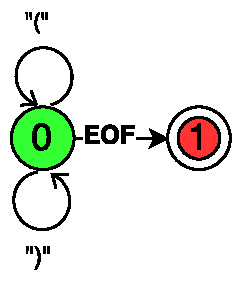
\includegraphics[width=5cm]{pics/ExampleInputGraph.pdf}
 \caption{Конечный автомат, подаваемый на вход анализатору }
 \label{InputGraph}
\end{figure}

В результате работы описанного алгоритма построено сжатое представление леса разбора, представленное на рис.~\ref{ExSppf}. Циклы в сжатом представлении леса разбора отображают наличие циклов во входном конечном автомате и позволяют извлекать потенциально бесконечное множество деревьев, каждое из которых соответствует цепочке, порождаемой автоматом.

\begin{figure}
 \centering
 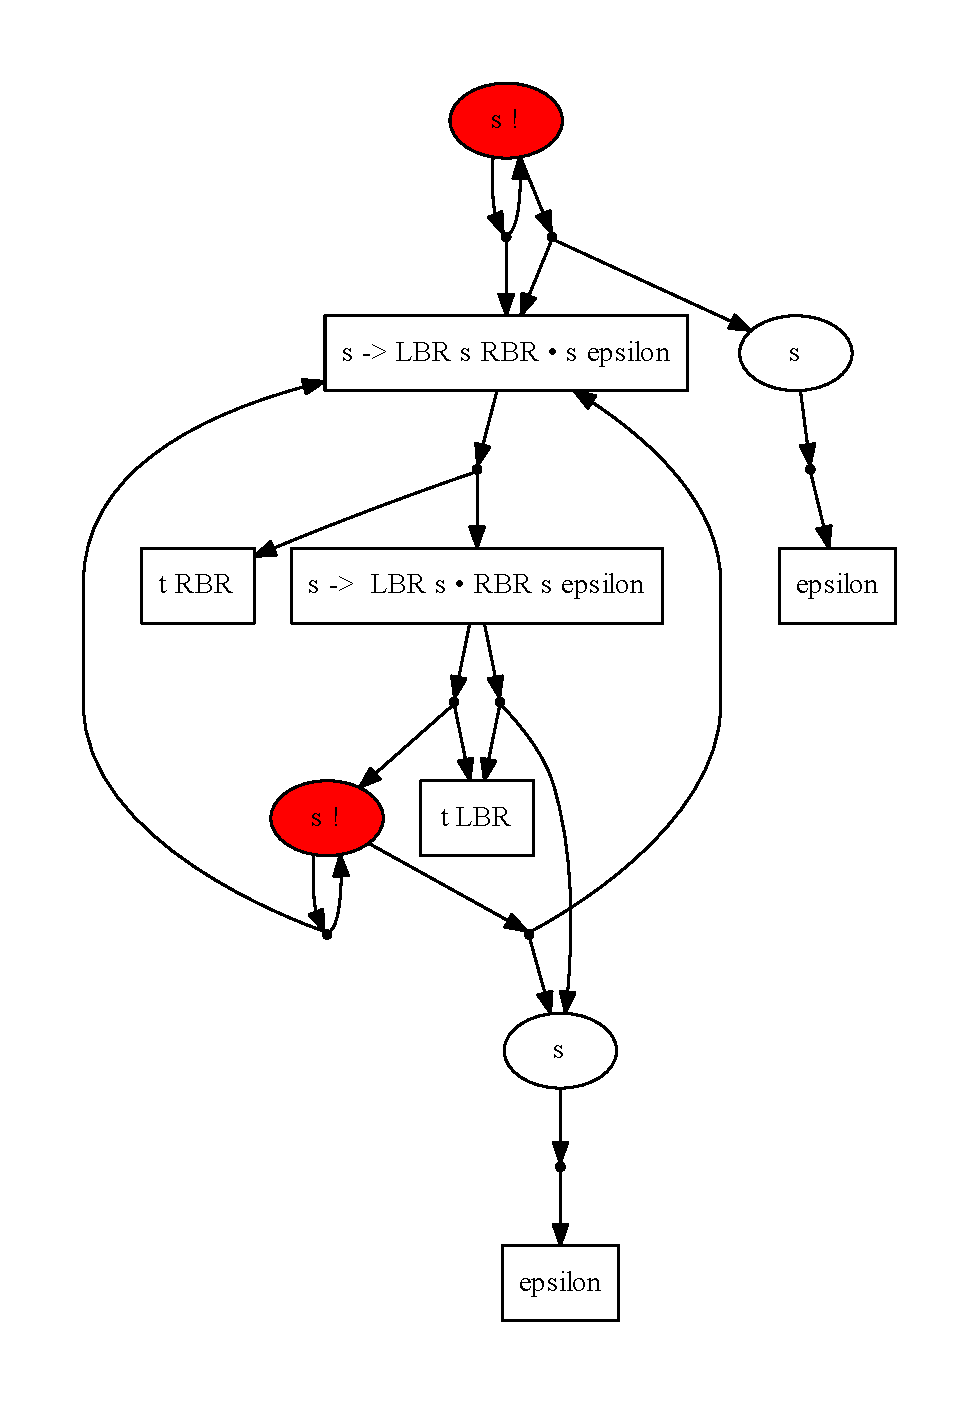
\includegraphics[width=13cm]{pics/SppfExample.pdf}
 \caption{Сжатое представление леса разбора для грамматики $G_4$ и конечного автомата на рис.~\ref{InputGraph} }
 \label{ExSppf}
\end{figure}

\subsection{Доказательство корректности}
Для того чтобы показать, что предложенный алгоритм работает корректно сначала нужно доказать, что процесс останавливается.

\textsc{Теорема 1.} 
\textit{Алгоритм завершает свою работу для произвольного детерминированного конечного автомата и контекстно-свободной грамматики.}

\textsc{Доказательство.}

Алгоритм завершает свою работу как только очередь дескрипторов становится пустой. Дескриптор с определённым набором значений полей в очередь добавляется лишь единожды. Таким образом, чтобы показать завершаемость алгоритма достаточно доказать, что количество дескрипторов конечно. 

Дескриптор состоит из четырёх элементов --- слот, индекс во входном потоке, вершина стека, дерево. Таким образом, общее количество дескрипторов не превышает прямого произведения возможного количества каждого из этих элементов. Количество индексов не больше количества вершин входного графа. Количество слотов конечно, потому что грамматика конечна. Вершина стека определяется парой --- слот и индекс, и значит тоже конечно. Часть леса, хранимая в дескрипторе, определяется однозначно именем нетерминала или слотом и двумя координатами во входном графе. Обе составляющие конечны. $\square$

Таким образом было показано, что количество дескрипторов --- конечное число.

\textsc{Определение 1.} 
\emph{Корректное дерево}~--- это упорядоченное дерево со следующими свойствами.
\begin{enumerate}
  \item Корень дерева соответствует стартовому нетерминалу грамматики $G$.
  \item Листья соответствуют терминалам грамматики $G$. Упорядоченная последовательность листьев соответствует некоторому пути во входном графе.
  \item Внутренние узлы соответствуют нетерминалам грамматики $G$. Потомки внутреннего узла (для нетерминала $N$) соответствуют символам правой части некоторой продукции для $N$ в грамматике $G$.
\end{enumerate}

Для того, чтобы доказать, что SPPF содержит только корректные деревья, сначала необходимо доказать следующую лемму.

\textsc{Лемма 1.} 
\textit{Для любой части леса $t$, построенного в процессе вывода, существует путь в графе $р$, такой что крона $t$ покрывает этот путь. }

\textsc{Доказательство.}

Для доказательство используется индукция по построению SPPF. 

\textsc{База.}

Для терминальных узлов утверждение очевидно. Терминальный узел соответствует ровно одному ребру во входном графе и строится только после прохода по этому ребру. Построение эпсилон узлов никак не зависит от входного графа, а производится только в соответствии с грамматикой. 

\textsc{Переход.}

Достаточно доказать для упакованных ячеек, всё остальное доказывается аналогично. Создание упакованных ячеек происходит в двух случаях --- при чтении нового терминала из входного потока или изъятии вершины стека, что значит, что текущий нетерминал был разобран и необходимо вернуться к точке, с которой этот разбор начался. 

Рассмотрим первый случай. У нас есть часть леса, которая соответствует какому-то пути $p$ в графе от вершины $v_0$ до $v_1$. Текущая позиция во входном потоке соответствует правой координате для этой части SPPF. При считывании нового терминала, создаётся упакованная ячейка, левым сыном которой становится уже построенная часть SPPF, а правым --- терминал. Получаем новую часть леса, соответствующее пути $P_1 = v_0 \dots v_1 v_{1+1}$.

Рассмотрим второй случай --- изъятие вершины со стека. Первая часть леса разбора Т1 хранится на ребре стека. Вторая часть Т2 построена по только что разобранному правилу. Каждая из этих частей соответствует какому-то подпути в графе и необходимо показать, что правая координата T1 совпадает с левой координатой T2. Это соответствует тому факту, что объединение этих частей леса даст часть леса, покрывающую путь в графе без дыр, то есть если в графе была цепочка {\it ``abcd''} и T1 соответствует {\it ``ab''}, то T2 будет соответствовать {\it ``bc''}. Для того, чтобы показать, что это условие выполняется, достаточно рассмотреть, как происходит процесс разбора. Как только в процессе обхода грамматики (в слоте) встречается нетерминал, создаётся новая вершина стека, которая хранит в себе слот с позицией за этим нетерминалом, на ребре хранится уже построенная часть леса. Правая координата этой части SPPF является номером вершины, с которой будет происходить дальнейший разбор, это число и записывается в новый дескриптор. Таким образом, после того, как нетерминал будет разобран до конца, будет создан новый упакованный узел, в котором в качестве левого потомка будет часть леса с ребра, а в качестве правого --- нетерминальный узел, левая координата которого совпадает с правой координатой левой части леса, так как именно с того места и начался разбор этого нетерминала. $\square$

Таким образом для упакованных узлов в дереве доказали необходимое. Доказательство для остальных видов узлов проводится аналогично.

\textsc{Теорема 2.} 
\textit{Любое дерево, извлечённое из SPPF, является корректным.}

\textsc{Доказательство.}

Рассмотрим произвольное извлечённое из SPPF дерево и докажем, что оно удовлетворяет определению. Первый и третий пункт определения корректного дерева следует из определения SPPF. 

Второй пункт следует из Леммы 1. Необходимо только показать, что такой путь начинается в начальной вершине и заканчивается в конечной. Действительно, так как работа алгоритма может быть начата только из начальной вершины, то левой координатой для неё будет стартовая вершина. Результатом работы алгоритма является SPPF. Узел помечается, как результирующий, если он помечен стартовым нетерминалом и его левая координата является стартовой вершиной, а правая --- финальной. $\square$

\textsc{Теорема 3.} 
\textit{Пусть грамматика Г порождает язык $L$. Тогда для каждого пути в графе $p$, соответствующего строке s из $L$, из SPPF может быть изъято корректное дерево.}

\textsc{Доказательство.}

Необходимо доказать, что SPPF содержит все корректные деревья вывода для всех корректных цепочек из входа. Как только процесс разбора начинается, в очередь дескрипторов добавляются дескрипторы для всех альтернатив стартового правила, соответствующие терминалу во входном потоке. Аналогичная ситуация происходит, как только в грамматике встречается нетерминал. Рассматриваются все альтернативы нетерминала и добавляются те, по которым может быть продолжен синтаксический анализ в соответствии со входным символом. Это гарантирует, что все альтернативы в выводе будут рассмотрены. При этом во входном графе все пути, соответствующие входным цепочкам, тоже рассматриваются, так как переход по ребру осуществляется всегда, если оно продолжает корректный префикс.$\square$

\subsection{Анализ данных большого объёма}
Одной из задач, сформулированных в данной работе, является использование предложенного алгоритма для анализа больших данных. Это востребовано, например, в задачах биоинформатики. Прежде чем формулировать задачу, следует ввести основные определения.

Исследование геномов является одной из распространённых задач биоинформатики. Информацию, содержащуюся в геноме можно представить в виде последовательностей символов и в дальнейшем эти последовательности анализировать. Геномы извлекаются из ДНК и позволяют характеризовать тот или иной организм. Для этого из генома необходимо выделить определённые участки, позволяющие сделать выводы о его свойствах. Геном (последовательность ДНК) --- строка в алфавите $\{A, C, G, T\}$, однозначно определяющая организм (или штамм), к которому она относится. Сборка --- набор подстрок генома, длина которых на порядки меньше длины самого генома. Метагеномная сборка --- смесь сборок нескольких геномов, то есть набор небольших подстрок нескольких геномов. Поскольку геном состоит из повторяющихся участков, то его можно представить в виде конечного автомата с последовательностями символов на рёбрах, который на практике часто представляется в виде графа  Де Брауна~\cite{Bruijn}.

Как упоминалось ранее, для решения задач, возникающих в биоинформатике, не нужно структурное представление вывода. Это значит, что дерево разбора, которое является результатом работы синтаксического анализатора, не нужно. Нужно лишь ответить на вопрос: порождает ли входной автомат данную подстроку или нет и вернуть координаты участка, на котором это происходит. При этом геном можно описать с помощью грамматики, т.е. про подцепочки, порождаемые входным конечным автоматом, известно, что они описываются некоторой грамматикой. Необходимо найти подавтоматы, принимающие цепочки, задаваемые некоторой грамматикой. Таким образом, предложенный алгоритм необходимо модифицировать таким образом, чтобы он решал данную задачу. 

Для решения поставленной задачи не нужно строить лес разбора, поэтому от функций для его построения можно просто отказаться. Самое простое представление результата --- набор путей. Однако для больших графов это может потребовать больших дополнительных расходов памяти. Чтобы этого избежать, можно предложить следующий подход: строить множество начальных и конечных вершин и контролировать длину путей. Это можно делать в процессе анализа, не накапливая дополнительной информации. Тогда после завершения работы можно будет выделить подграф, который, возможно, будет содержать лишние пути и потому потребуется его последующая обработка с накоплением путей. При этом извлечённые подграфы будут существенно меньше исходного графа и их повторная обработка не сильно сказывается на производительности.

Таким образом, в местах, где раньше в алгоритме строились узлы дерева, теперь просто запоминаются координаты. Вместо хранения поддерева на рёбрах стека теперь хранится просто число --- начало и конец подцепочки, созданной на момент создания вершины стека. Кроме координат начала и конца и длины можно ещё сохранять путь целиком. Для этого на рёбрах нужно просто сохранять цепочки, а не одно число. 

\section{Реализация}
Предложенный алгоритм был реализован в рамках исследовательского проекта YaccConstructor. В данной главе описывается архитектура предложенного решения: основные модули и их взаимодействие. Кроме того, рассматриваются особенности практической реализации.

\subsection{Архитектура предложенного решения}
На основе предложенного алгоритма разработан новый модуль инструмента YaccConstructor, который является генератором в терминах, принятых в этом проекте. Это показано на рис.~\ref{Arch}, где изображена архитектура инструмента YaccConstructor и цветом выделен реализованный модуль.

\begin{figure}[h]
 \centering
 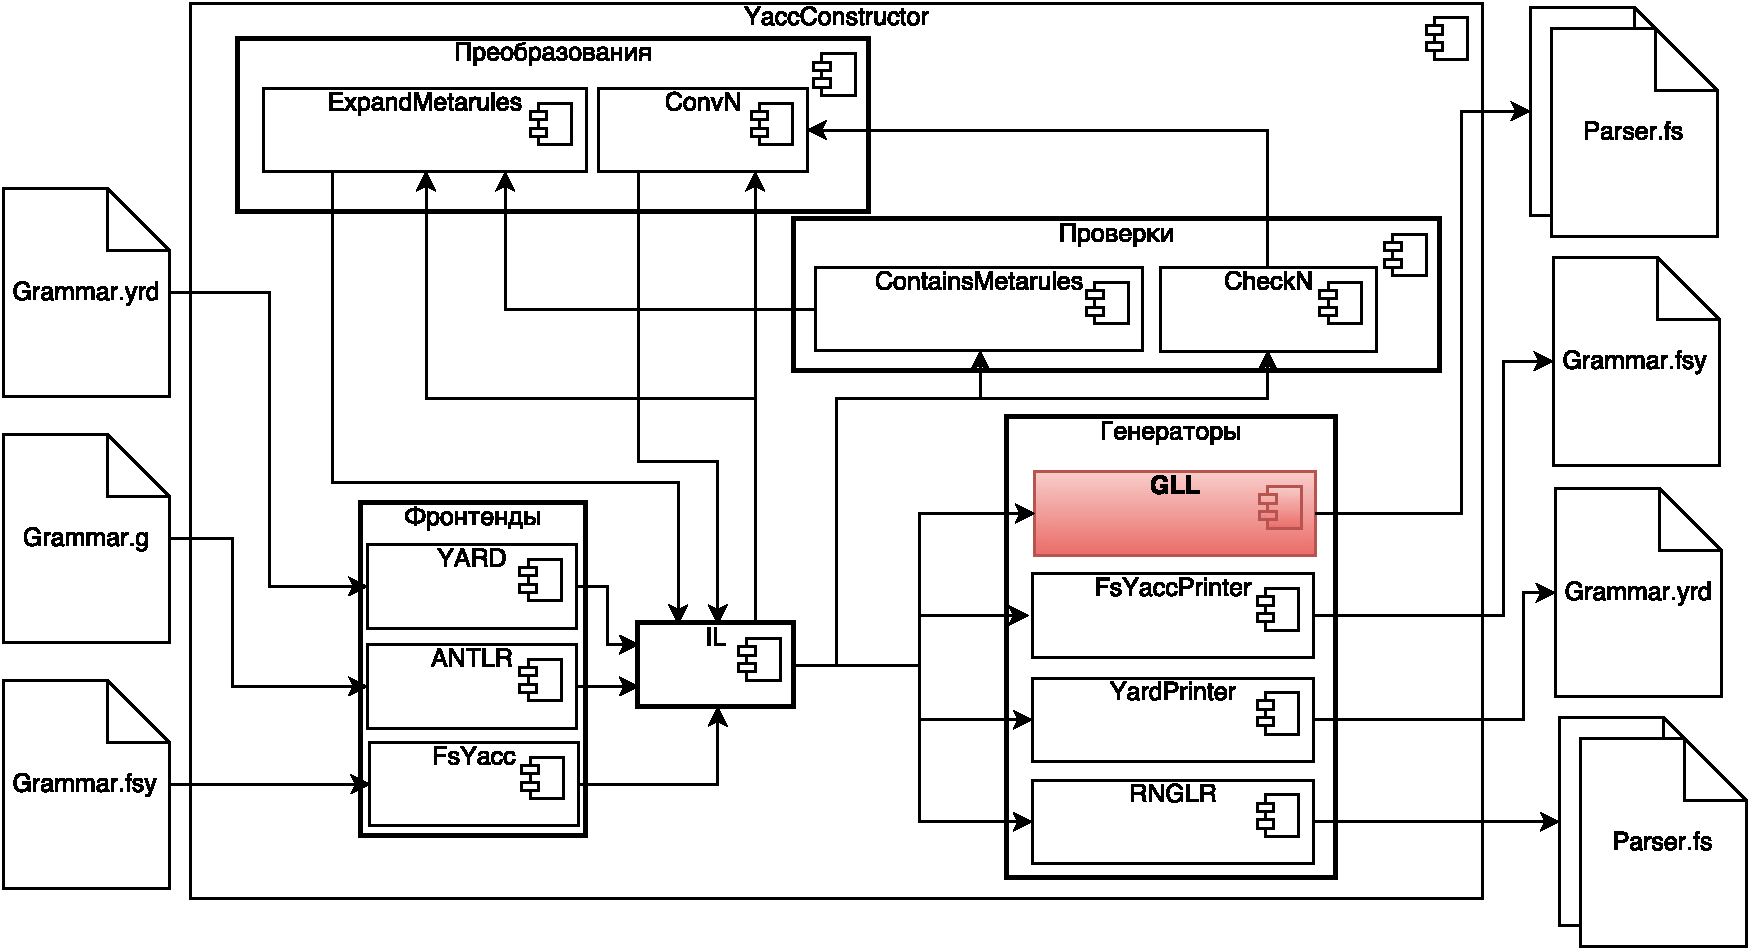
\includegraphics[width=15cm]{pics/Arch.pdf}
 \caption{Архитектура инструмента YaccConstructor (рисунок взят из работы~\cite{GrigorievPhd})}
 \label{Arch}
\end{figure}

Внутреннее устройство этого модуля показано на рис.~\ref{Arch2}. Основными компонентами являются генератор, который по грамматике строит управляющие таблицы и дополнительные структуры данных, компонента с описанием SPPF и функциями работы с ним, два интерпретатора управляющих таблиц, различающиеся тем, что один из них строит лес разбора, а другой нет. Интерпретаторы разделены в силу того, что структуры для хранения элементов дерева тесно связаны с другими структурами, используемыми при анализе, например, стеком, а отказ от построения леса был вызван необходимостью получить алгоритм, расходующий меньше памяти. По этой причине реализовано два набора структур данных, каждая из которых оптимальна при решении соответствующей задачи.

На вход генератор принимает внутреннее представление в формате IL, которое строится по грамматике и может быть получено с помощью соответствующего фронтенда. Так как в язык описания грамматики позволяет использовать конструкции, которые не обрабатываются генератором (например, метапрвила), то необходимо применить соответствующие преобразования, что достигается заданием специальных параметров при запуске инструмента. Результатом работы генератора является файл с исходным кодом, в котором описаны управляющие таблицы и вспомогательная информация, которая в дальнейшем используется интерпретатором. 

Интерпретатор написан вручную и содержит в себе основную логику алгоритма. Он подключается в виде отдельной сборки к целевому приложению и позволяет на основе сгенерированнх данных выполнять анализ входа.

Пользователь при создании приложения, использующего модуль, добавляет в свой проект сгенерированный файл, ссылку на интерпретатор и файл, содержащий лексический анализатор (полученный с помощью другого модуля YC, который не описывается в данной работе) и вызывает соответствующую функцию для синтаксического анализа. Результатом работы такой функции является либо SPPF, либо набор координат во входном графе, позволяющих определить положение в нём участка, порождающего строку, принимаемую соответствующей грамматикой.

\begin{figure}
 \centering
 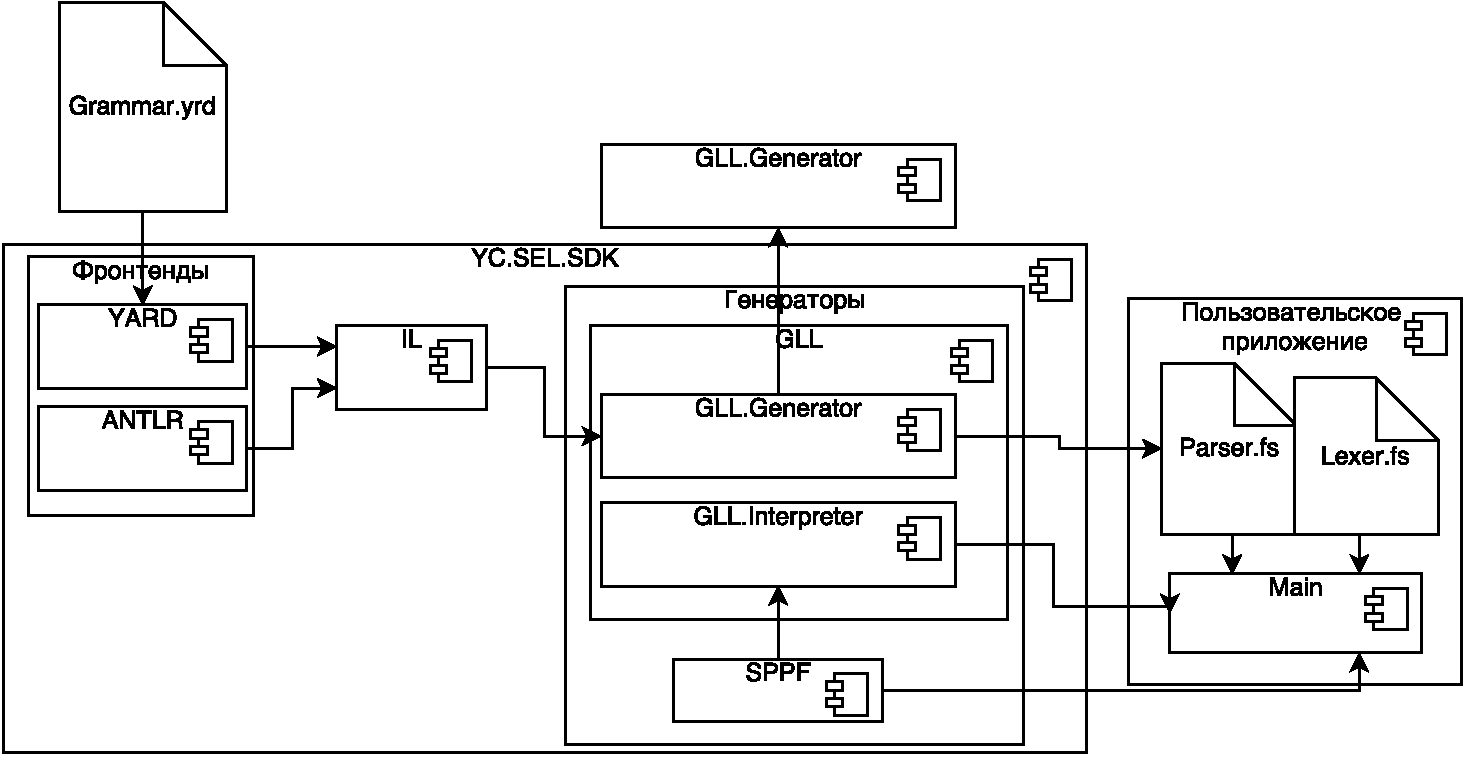
\includegraphics[width=15cm]{pics/GLL_Proc.pdf}
 \caption{Принцип работы реализованного модуля (рисунок взят и модифицирован из работы~\cite{GrigorievPhd})}
 \label{Arch2}
\end{figure}

\subsection{Особенности используемых структур данных}
Алгоритм реализован в рамках проекта YaccConstructor на языке программирования F\#. Исходный код свободно доступен в репозитории \url{https://github.com/YaccConstructor/YaccConstructor}, автор вёл разработку под учётной записью {\it AnastasiyaRagozina}.

Заявленная производительность алгоритма --- в худшем случае куб по памяти и времени --- обоснована теоретически~\cite{Johnstone201564}. На практике же, для достижения высокой производительности алгоритма, написанного с использованием языков высокого уровня, необходимо приложить некоторые усилия. Рассуждениям на данную тему и описанию эффективных структур данных посвящена работа~\cite{Johnstone2011}. При реализации описанного алгоритма подобные проблемы так же возникли: высокий расход памяти и медленные структуры данных. Основной проблемой было хранение леса разбора и поиск уже существующих узлов. Хранение узлов в многомерных массивах, как было предложено в ~\cite{Johnstone2011}, накладывало значительные ограничения на длину входа. Кроме того, хранение в каждом узле дерева нескольких чисел (имени нетерминала и координаты начала и конца подцепочки, соответствующей данному поддереву) делало его громоздким. В результате, для того, чтобы уменьшить расход памяти при хранении SPPF было использовано сжатие хранимых в узлах координат в одно число. Это позволило вместо хранения двух чисел хранить одно, которое можно было использовать в качестве ключа при поиске уже созданных поддеревьев. Аналогичное сжатие использовалось для хранения слотов. Для хранения терминальных узлов в алгоритме было предложено использовать динамически изменяемый массив,  размер которого сравним с размером входных данных, что приводит к выделению большого количества лишней памяти при использовании стандартного типа \verb|ResizeArray<_>| при больших размерах входа. Для решения этой проблемы использовалась модификация динамически изменяемого массива, в которой память выделяется блоками константного размера. Данная структура данных была реализована в рамках работы над RNGLR-алгоритмом. В рамках данной работы она была выделена в библиотеку структур данных \texttt{FSharpx.Collections}, поддерживаемую FSharp-сообществом~\cite{FsharpX}. Подобные задачи являются интересными с инженерной точки зрения и часто возникают на практике.

Важной задачей так же является представление метагеномной сборки и её обработка, так как, в отличие от графа, являющегося аппроксимацией встроенных языков, граф, представляющего метагеномную сборку, как правило, существенно большего размера. Для того, чтобы уменьшить размер самого графа, на рёбрах хранится не по одному токену, а цепочки токенов. Это приводит к тому, что теперь в качестве координаты начала и конца подстроки используется не два числа, а четыре --- номера рёбер и позиция на них. По аналогии, эти числа сжимались. Для того, чтобы эффективно использовать такие индексы была создана структура данных, доступ к элементам которой как у массива, но по сжатому числу. 

При обработке графа метагеномной сборки были использованы следующие знания о его структуре и особенностях решаемой задачи. В графе есть рёбра, на которых лежат подстроки длины большей, чем длина искомой подстроки. Это означает, что такие рёбра можно удалить из графа и обработать отдельно, как линейные данные. При этом граф распадается на набор связанных компонент, что позволяет обрабатывать части входного графа полностью независимо. Это, в свою очередь, существенно упрощает параллельную обработку данных: возникает классическая параллельность по данным, когда к большому количеству независимых данных нужно применить одну и ту же функцию обработки. 

Однако, несмотря на то, что параллельность по данным может быть реализована очевидным образом, использование нескольких потоков в рамках одного многоядерного процессора не даёт ожидаемого прироста производительности, что наглядно продемонстрировано на рис.~\ref{StackExp}.

\begin{figure}
 \centering
 \includegraphics[width=15cm]{pics/Stack.eps}
 \caption{Сравнение производительности предложенного решения при запуске на нескольких потоках }
 \label{StackExp}
\end{figure} 

Замеры, результаты которых представлены на рис.~\ref{StackExp} и рис.~\ref{StackExp2} проводились на машине со следующей конфигурацией:
\begin{itemize}
\item OS Name	Microsoft Windows 10 Pro
\item System Type x64-based PC
\item Processor	Intel(R) Core(TM) i7-4790 CPU 3.60GHz, 3601 Mhz, 4 Core(s), 4 Logical Processor(s)
\item Installed Physical Memory (RAM)	32.0 GB
\end{itemize}

Из рис.~\ref{StackExp} видно, что максимальная производительность наблюдается при использовании двух потоков. Однако прирост производительности по сравнению с использованием одного потока составляет всего 6.4\%, что значительно меньше теоретически возможного.

Такое поведение системы связано с тем, что при обработке одного графа происходит активное обращение к вспомогательным структурам данных большого объёма. При этом обращения, в силу особенностей алгоритма, плохо локализованы. В связи с чем, при попытке обработать несколько графов одновременно на одном процессоре, учащаются промахи кэшей. Частично решить эту проблему удалось заменив очередь дескрипторов на стек, это сделало обращения к данным более локализованными и позволило улучшить производительность решения. 

Результаты измерений после замены очереди на стек представлены на рис.~\ref{StackExp2}. Максимальная производительность достигается при использовании трёх потоков и прирост производительность составляет 14.2\%. На рис.~\ref{StackExp2} представлено сравнение производительности до и после модификации.



\begin{figure}
 \centering
 \includegraphics[width=15cm]{pics/StackVSQueue.eps}
 \caption{Сравнение производительности предложенного решения замене стека на очередь для хранения дескрипторов }
 \label{StackExp2}
\end{figure}

Для того, чтобы избавиться от проблем с кэшами при многопоточной обработке, можно использовать многопроцессорные системы, такие как вычислительные кластеры. При этом, как показали проведённые ранее эксперименты, имеет смысл запускать не более двух потоков на одном процессоре. Так как время обработки одного подграфа занимает время порядка нескольких секунд, то затраты на передачу по сети не должны заметно уменьшать выигрыш, получаемый за счёт параллельной обработки при достаточном количестве графов для обработки на одном узле.  

Для реализации вычислений в кластере была выбрана технология MBrace, которое позволяет, с одной стороны, управлять кластером в облаке Microsoft.Azure с помощью скриптов на F\#. Предоставляется полный набор функций, позволяющий сконфигурировать кластер ``с нуля'', а затем управлять им (например, изменять количество машин). С другой стороны, MBrace позволяет прозрачно использовать кластер в коде на F\#. Это достигается благодаря предоставлению набора высокоуровневых функций и окружения \texttt{cloud}, благодаря которому код, предназначенный для выполнения в кластере можно задать следующим образом.

\begin{listing}
    \begin{pyglist}[language=ocaml,numbers=left,numbersep=5pt]
    
let parallelTask = 
    [ for i in 1 .. 10 -> 
          cloud { return sprintf "i'm work item %d" i } ]
    |> Cloud.Parallel
    |> cluster.CreateProcess

\end{pyglist}
\caption{Код для запуска предложенного решения в кластере}
\label{lst:mbraceExample}
\end{listing}

В скобках \verb|cloud { }| может находиться произвольный код на F\#. Все необходимые для выполнения этого кода в кластере дополнительные действия и коммуникации (передача данных, подготовка и передача бинарных файлов) осуществляется автоматически и не требует участия разработчика. Таким образом, в предположении, что функция обработки графа \texttt{processGraph}  реализована и всё, что необходимо для реализации обработки массива графов о кластере, это ``завернуть'' её вызов в окружение \texttt{cloud} следующим образом.

\begin{listing}
    \begin{pyglist}[language=ocaml,numbers=left,numbersep=5pt]
    
let parallelGraphProcessing graphs = 
    [ for g in graphs -> cloud { return processGraph g } ]
    |> Cloud.Parallel
    |> cluster.CreateProcess

\end{pyglist}
\caption{Код для запуска предложенного решения в кластере с параметризацией входных данных}
\label{lst:mbraceExample}
\end{listing}

\section{Эксперименты}
В рамках данной работы были произведены эксперименты по сравнению алгоритмов синтаксического анализа регулярных множеств для на основе алгоритма RNGLR и GLL. 

Замеры производились на компьютере со следующими характеристиками.
\begin{itemize}
\item Операционная система: Microsoft Windows 8.1 Pro.
\item Тип системы: х64-based PC.
\item Процессор: Intel(R) Core(TM) i7-4790 CPU 3.60GHz, 3601 Mhz, 4 Core(s), 8 Logical Processor(s).
\item Объём оперативной памяти: 16.0 GB.
\end{itemize}

Для сравнения были выбраны несколько грамматик, представляющих как практический, так и теоретический интерес. Одна из таких грамматик --- сильно неоднозначная грамматика $G_5$ (листинг~\ref{grmG5}), реализующая худший случай для анализатора, и позволяющая оценить производительность алгоритмов в задачах биоинформатики, так как большинство шаблонов в них являются сильно неоднозначными. Результаты измерений представлены на рис.~\ref{exp1}. 

\begin{listing}
\caption{Грамматика $G_5$}
\label{grmG5}
\centering
$\begin{array}{rl}
s \rightarrow s \ s \ s \ |  \ s \ s \ | \ B 
\end{array}$
\end{listing} 

\begin{figure}
 \centering
 \includegraphics[width=15cm]{pics/UmbLog.eps}
 \caption{Сравнение времени работы решений на основе алгоритмов GLL и RNGLR для грамматики $G_5$}
 \label{exp1}
\end{figure}

Следующей рассматриваемой грамматикой является неоднозначная грамматика правильных скобочных последовательностей $G_6$ (листинг ~\ref{grmG6}). Данная грамматика представляет интерес с практический точки зрения, так как она близка к шаблонам для поиска, используемым в задачах биоинформатики. 

\begin{listing}
\caption{Грамматика $G_6$}
\label{grmG6}
\centering
$\begin{array}{rl}
s \rightarrow s \ s \ |  \ LBR \ s \ RBR \ | \ \varepsilon 
\end{array}$
\end{listing}

Результаты измерений представлены на рис.~\ref{exp2}. Видно, что время работы алгоритма на основе RNGLR растёт значительно быстрее, чем алгоритма на основе GLL, с ростом длины входной цепочки. 

\begin{figure}
 \centering
 \includegraphics[width=15cm]{pics/Brs.eps}
 \caption{Сравнение времени работы решений на основе алгоритмов GLL и RNGLR для грамматики $G_6$}
 \label{exp2}
\end{figure}

Следующий эксперимент производился на грамматике подмножества языка T-SQL~\cite{YCZOO} . Входные графы строились с помощью последовательной конкатенации блоков с параллельными путями, которые соответствуют использованию операторов ветвления при построении выражения. Пример входного графа приведён на рис.~\ref{SQLInp}.

\begin{figure}
 \centering
 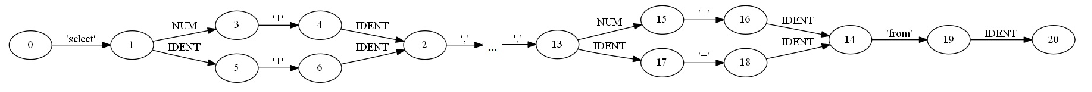
\includegraphics[width=15cm]{pics/SQLInput}
 \caption{Структура графа для экспериментов на грамматике T-SQL}
 \label{SQLInp}
\end{figure}

\begin{figure}
 \centering
 \includegraphics[width=15cm]{pics/SQL.eps}
 \caption{Сравнение времени работы решений на основе алгоритмов GLL и RNGLR для грамматики T-SQL}
 \label{exp3}
\end{figure}

Результаты измерений приведены на рис.~\ref{exp3} В данном случае GLL оказался медленнее. Однако необходимо заметить, что, с одной стороны, на входах практически значимой длины замедление несущественно, а с другой, алгоритм на основе GLR длительное время оптимизировался. Техническая доработка GLL может позволить улучшить его производительность.

Также было проведено сравнение алгоритмов на основе RNGLR и GLL на задаче поиска подцепочки в геноме. В качестве искомой подцепочки была выбрана транспортная РНК, шаблон для поиска которой был описан грамматикой, представленной на листинге~\ref{lst:csqlExample}. Данная грамматика является сильно неоднозначной. В качестве входа была выбрана последовательность из тестов инструмента Infernal~\cite{Infernal} от которой последовательно брались участки длины $100 + 10*k$, начинающиеся с нулевой позиции. Таким образом был получен набор тестовых данных: множество цепочек с увеличивающейся длиной.

\begin{listing}
    \begin{pyglist}[language=ocaml,numbers=left,numbersep=5pt]

stem<s>: 
      A stem<s> U
    | U stem<s> A
    | C stem<s> G
    | G stem<s> C
    | G stem<s> U
    | U stem<s> G
    | s

any: A | U | G | C

[<Start>]
full: folded any?

a_5_8 : any*[5..8]
a_1_3 : any*[1..3]

folded: stem<(a_1_3 stem<any*[7..10]> 
              a_1_3 stem<a_5_8> 
              any*[3..6] 
              stem<a_5_8>)> 

\end{pyglist}
\caption{Пример грамматики для описания транспортной РНК}
\label{lst:csqlExample}
\end{listing}

\begin{figure}
 \centering
 \includegraphics[width=15cm]{pics/BioLog.eps}
 \caption{Сравнение времени работы решений на основе алгоритмов GLL и RNGLR для грамматики на листинге~\ref{lst:csqlExample}}
 \label{fig:Stack}
\end{figure}

График зависимости времени работы от длины цепочки приведён на рис.~\ref{fig:Stack}. Для RNGLR приведены первые 10 замеров, так как дальнейшие измерения для алгоритма на основе RNGLR было решено прекратить из-за его низкой производительности. Приведённые результаты показывают, что реализованный в рамках данной работы алгоритм более чем в 400 раз быстрее алгоритма на основе RNGLR, что согласуется с результатами сравнений на сильно неоднозначной грамматике.

\section*{Заключение}
В данной работе получены следующие результаты.
\begin{itemize}
\item Разработан алгоритм синтаксического анализа динамически  формируемого кода на основе алгоритма GLL, результатом работы которого является лес разбора, который компактно представляется с помощью структуры данных SPPF.
\item Доказана корректность и завершаемость предложенного алгоритма.
\item Предложенный алгоритм реализован на языке F\# в виде модуля инструмента YaccConstructor. Исходный код доступен в репозитории YaccConstructor~\cite{YCUrl}, автор работал под учётной записью \textit{AnastasiyaRagozina}.
\item Проведён ряд экспериментов и выполнено сравнение с алгоритмом, реализующим аналогичный подход.
\item Выполнена модификация предложенного алгоритма, позволяющая обрабатывать входные данные большого размера, что продемонстрировано на примере поиска подпоследовательностей в метагеномных сборках.
\end{itemize}

По результатам работы сделан доклад ``Обобщённый табличный LL-анализ'' на конференции ``ТМПА-2014'', тезисы опубликованы в сборнике материалов конференции,  и выполнена  публикация ``Средство разработки инструментов статического анализа встроенных языков'' в сборнике ``Наука и инновации в технических университетах материалы Восьмого Всероссийского форума студентов, аспирантов и молодых ученых''. Исследовательская работа поддержана грантом УМНИК: договор \textnumero 5609ГУ1/2014.

Существует несколько направлений дальнейшего развития полученных результатов. Во-первых, важной задачей является оценка теоретической сложности представленного алгоритма. Во-вторых, необходимо исследовать возможности по непосредственной поддержке грамматик в EBNF и поддержке булевых грамматик. Использование булевых, или даже конъюнктивных, грамматик позволит более точно задавать критерии поиска, например, это позволит специфицировать высоту \texttt{stem}-а. Эта возможность продемонстрирована в листинге~\ref{lst:conjExample}: правило \verb|stem_3_5<s>| описывает \texttt{stem} высотой от 3 до 5 пар.

%\fvset{frame=lines,framesep=5pt}
\begin{listing}
    \begin{pyglist}[language=ocaml,numbers=left,numbersep=5pt]

stem<s>: 
      A stem<s> U
    | U stem<s> A
    | C stem<s> G
    | G stem<s> C
    | G stem<s> U
    | U stem<s> G
    | s

any: A | U | G | C
stem_3_5<s>: stem <s> & (any*[3..5] s any*[3..5])

\end{pyglist}
\caption{Пример конъюнктивной грамматики для описания stem-ов фиксированной высоты}
\label{lst:conjExample}
\end{listing}


Кроме этого, необходимо выполнить ряд технических доработок, таких как оптимизация реализации.

\setmonofont[Mapping=tex-text]{CMU Typewriter Text}
\bibliographystyle{ugost2008ls}
\bibliography{biblio.bib}
\end{document}
